% Created by tikzDevice version 0.12.3 on 2020-05-11 12:49:51
% !TEX encoding = UTF-8 Unicode
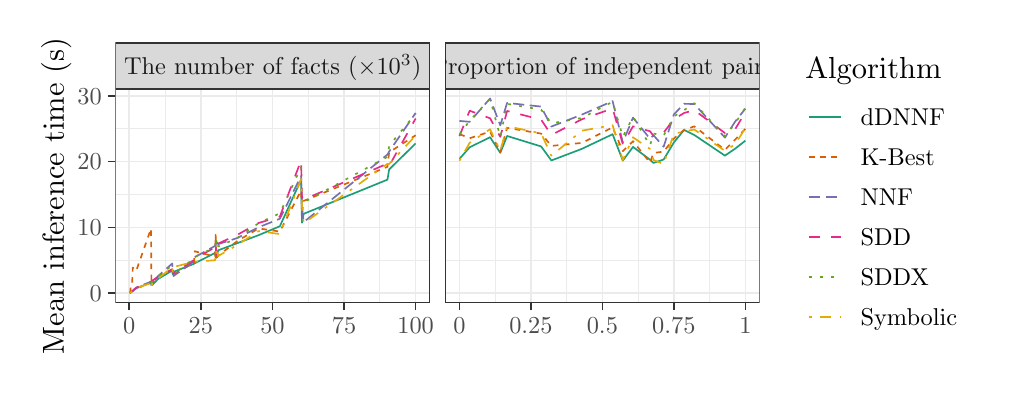
\begin{tikzpicture}[x=1pt,y=1pt]
\definecolor{fillColor}{RGB}{255,255,255}
\path[use as bounding box,fill=fillColor,fill opacity=0.00] (0,0) rectangle (346.90,130.09);
\begin{scope}
\path[clip] (  0.00,  0.00) rectangle (346.90,130.09);
\definecolor{drawColor}{RGB}{255,255,255}
\definecolor{fillColor}{RGB}{255,255,255}

\path[draw=drawColor,line width= 0.6pt,line join=round,line cap=round,fill=fillColor] (  0.00,  0.00) rectangle (346.90,130.09);
\end{scope}
\begin{scope}
\path[clip] ( 31.71, 30.69) rectangle (145.35,108.01);
\definecolor{fillColor}{RGB}{255,255,255}

\path[fill=fillColor] ( 31.71, 30.69) rectangle (145.35,108.01);
\definecolor{drawColor}{gray}{0.92}

\path[draw=drawColor,line width= 0.3pt,line join=round] ( 31.71, 46.03) --
	(145.35, 46.03);

\path[draw=drawColor,line width= 0.3pt,line join=round] ( 31.71, 69.81) --
	(145.35, 69.81);

\path[draw=drawColor,line width= 0.3pt,line join=round] ( 31.71, 93.59) --
	(145.35, 93.59);

\path[draw=drawColor,line width= 0.3pt,line join=round] ( 49.66, 30.69) --
	( 49.66,108.01);

\path[draw=drawColor,line width= 0.3pt,line join=round] ( 75.52, 30.69) --
	( 75.52,108.01);

\path[draw=drawColor,line width= 0.3pt,line join=round] (101.39, 30.69) --
	(101.39,108.01);

\path[draw=drawColor,line width= 0.3pt,line join=round] (127.25, 30.69) --
	(127.25,108.01);

\path[draw=drawColor,line width= 0.6pt,line join=round] ( 31.71, 34.14) --
	(145.35, 34.14);

\path[draw=drawColor,line width= 0.6pt,line join=round] ( 31.71, 57.92) --
	(145.35, 57.92);

\path[draw=drawColor,line width= 0.6pt,line join=round] ( 31.71, 81.70) --
	(145.35, 81.70);

\path[draw=drawColor,line width= 0.6pt,line join=round] ( 31.71,105.48) --
	(145.35,105.48);

\path[draw=drawColor,line width= 0.6pt,line join=round] ( 36.72, 30.69) --
	( 36.72,108.01);

\path[draw=drawColor,line width= 0.6pt,line join=round] ( 62.59, 30.69) --
	( 62.59,108.01);

\path[draw=drawColor,line width= 0.6pt,line join=round] ( 88.46, 30.69) --
	( 88.46,108.01);

\path[draw=drawColor,line width= 0.6pt,line join=round] (114.32, 30.69) --
	(114.32,108.01);

\path[draw=drawColor,line width= 0.6pt,line join=round] (140.19, 30.69) --
	(140.19,108.01);
\definecolor{drawColor}{RGB}{27,158,119}

\path[draw=drawColor,line width= 0.6pt,line join=round] ( 36.88, 34.20) --
	( 37.03, 34.26) --
	( 37.34, 34.43) --
	( 37.76, 34.78) --
	( 37.96, 34.89) --
	( 39.21, 35.94) --
	( 44.56, 37.96) --
	( 44.72, 37.05) --
	( 45.03, 37.14) --
	( 47.07, 39.24) --
	( 52.24, 42.35) --
	( 52.40, 40.98) --
	( 52.71, 41.86) --
	( 60.08, 44.75) --
	( 60.39, 44.97) --
	( 67.76, 48.70) --
	( 67.92, 47.86) --
	( 68.07, 47.05) --
	( 68.23, 47.32) --
	( 68.85, 49.64) --
	( 75.75, 52.22) --
	( 83.44, 55.11) --
	( 91.12, 58.33) --
	( 98.80, 75.16) --
	( 99.11, 59.59) --
	( 99.73, 62.82) --
	(130.00, 75.17) --
	(130.62, 78.87) --
	(140.19, 88.26);
\definecolor{drawColor}{RGB}{217,95,2}

\path[draw=drawColor,line width= 0.6pt,dash pattern=on 2pt off 2pt ,line join=round] ( 36.88, 34.22) --
	( 37.03, 34.33) --
	( 37.34, 37.18) --
	( 37.76, 37.64) --
	( 37.96, 43.41) --
	( 39.21, 42.20) --
	( 44.56, 57.46) --
	( 44.72, 36.84) --
	( 45.03, 37.68) --
	( 47.07, 40.19) --
	( 52.24, 42.81) --
	( 52.40, 41.77) --
	( 52.71, 40.98) --
	( 60.08, 45.16) --
	( 60.39, 49.30) --
	( 67.76, 47.31) --
	( 67.92, 55.25) --
	( 68.07, 48.59) --
	( 68.23, 46.96) --
	( 68.85, 47.72) --
	( 75.75, 52.99) --
	( 83.44, 57.55) --
	( 91.12, 56.42) --
	( 98.80, 71.23) --
	( 99.11, 62.93) --
	( 99.73, 67.49) --
	(130.00, 79.80) --
	(130.62, 85.06) --
	(140.19, 91.20);
\definecolor{drawColor}{RGB}{117,112,179}

\path[draw=drawColor,line width= 0.6pt,dash pattern=on 4pt off 2pt ,line join=round] ( 36.88, 34.22) --
	( 37.03, 34.29) --
	( 37.34, 34.49) --
	( 37.76, 34.88) --
	( 37.96, 35.00) --
	( 39.21, 36.19) --
	( 44.56, 38.30) --
	( 44.72, 37.18) --
	( 45.03, 37.98) --
	( 47.07, 40.27) --
	( 52.24, 44.88) --
	( 52.40, 42.06) --
	( 52.71, 40.35) --
	( 60.08, 45.65) --
	( 60.39, 47.17) --
	( 67.76, 51.25) --
	( 67.92, 52.15) --
	( 68.07, 51.25) --
	( 68.23, 52.79) --
	( 68.85, 51.87) --
	( 75.75, 54.08) --
	( 83.44, 57.97) --
	( 91.12, 61.03) --
	( 98.80, 76.47) --
	( 99.11, 65.20) --
	( 99.73, 59.83) --
	(130.00, 84.23) --
	(130.62, 85.33) --
	(140.19, 99.28);
\definecolor{drawColor}{RGB}{231,41,138}

\path[draw=drawColor,line width= 0.6pt,dash pattern=on 4pt off 4pt ,line join=round] ( 36.88, 34.24) --
	( 37.03, 34.31) --
	( 37.34, 34.50) --
	( 37.76, 34.90) --
	( 37.96, 35.05) --
	( 39.21, 36.07) --
	( 44.56, 38.21) --
	( 44.72, 38.54) --
	( 45.03, 38.69) --
	( 47.07, 40.00) --
	( 52.24, 42.70) --
	( 52.40, 41.93) --
	( 52.71, 41.20) --
	( 60.08, 46.14) --
	( 60.39, 46.70) --
	( 67.76, 50.70) --
	( 67.92, 48.30) --
	( 68.07, 50.28) --
	( 68.23, 47.98) --
	( 68.85, 52.07) --
	( 75.75, 55.24) --
	( 83.44, 59.51) --
	( 91.12, 61.81) --
	( 98.80, 82.15) --
	( 99.11, 68.77) --
	( 99.73, 67.98) --
	(130.00, 80.96) --
	(130.62, 80.15) --
	(140.19, 97.28);
\definecolor{drawColor}{RGB}{102,166,30}

\path[draw=drawColor,line width= 0.6pt,dash pattern=on 1pt off 3pt ,line join=round] ( 36.88, 34.20) --
	( 37.03, 34.32) --
	( 37.34, 34.48) --
	( 37.76, 34.84) --
	( 37.96, 34.97) --
	( 39.21, 35.75) --
	( 44.56, 37.97) --
	( 44.72, 36.07) --
	( 45.03, 38.73) --
	( 47.07, 40.22) --
	( 52.24, 44.23) --
	( 52.40, 43.29) --
	( 52.71, 40.97) --
	( 60.08, 46.70) --
	( 60.39, 47.27) --
	( 67.76, 50.76) --
	( 67.92, 53.24) --
	( 68.07, 51.86) --
	( 68.23, 53.84) --
	( 68.85, 51.03) --
	( 75.75, 54.08) --
	( 83.44, 59.44) --
	( 91.12, 63.01) --
	( 98.80, 79.72) --
	( 99.11, 66.18) --
	( 99.73, 66.97) --
	(130.00, 83.43) --
	(130.62, 87.45) --
	(140.19, 98.97);
\definecolor{drawColor}{RGB}{230,171,2}

\path[draw=drawColor,line width= 0.6pt,dash pattern=on 1pt off 3pt on 4pt off 3pt ,line join=round] ( 36.88, 34.23) --
	( 37.03, 34.28) --
	( 37.34, 34.44) --
	( 37.76, 34.80) --
	( 37.96, 34.97) --
	( 39.21, 36.01) --
	( 44.56, 37.80) --
	( 44.72, 36.11) --
	( 45.03, 37.78) --
	( 47.07, 39.38) --
	( 52.24, 43.57) --
	( 52.40, 41.73) --
	( 52.71, 43.60) --
	( 60.08, 45.48) --
	( 60.39, 45.53) --
	( 67.76, 46.06) --
	( 67.92, 48.49) --
	( 68.07, 47.82) --
	( 68.23, 50.65) --
	( 68.85, 47.58) --
	( 75.75, 51.59) --
	( 83.44, 56.58) --
	( 91.12, 55.51) --
	( 98.80, 75.37) --
	( 99.11, 65.39) --
	( 99.73, 59.41) --
	(130.00, 80.88) --
	(130.62, 80.85) --
	(140.19, 91.13);
\definecolor{drawColor}{gray}{0.20}

\path[draw=drawColor,line width= 0.6pt,line join=round,line cap=round] ( 31.71, 30.69) rectangle (145.35,108.01);
\end{scope}
\begin{scope}
\path[clip] (150.85, 30.69) rectangle (264.49,108.01);
\definecolor{fillColor}{RGB}{255,255,255}

\path[fill=fillColor] (150.85, 30.69) rectangle (264.49,108.01);
\definecolor{drawColor}{gray}{0.92}

\path[draw=drawColor,line width= 0.3pt,line join=round] (150.85, 46.03) --
	(264.49, 46.03);

\path[draw=drawColor,line width= 0.3pt,line join=round] (150.85, 69.81) --
	(264.49, 69.81);

\path[draw=drawColor,line width= 0.3pt,line join=round] (150.85, 93.59) --
	(264.49, 93.59);

\path[draw=drawColor,line width= 0.3pt,line join=round] (168.93, 30.69) --
	(168.93,108.01);

\path[draw=drawColor,line width= 0.3pt,line join=round] (194.76, 30.69) --
	(194.76,108.01);

\path[draw=drawColor,line width= 0.3pt,line join=round] (220.59, 30.69) --
	(220.59,108.01);

\path[draw=drawColor,line width= 0.3pt,line join=round] (246.42, 30.69) --
	(246.42,108.01);

\path[draw=drawColor,line width= 0.6pt,line join=round] (150.85, 34.14) --
	(264.49, 34.14);

\path[draw=drawColor,line width= 0.6pt,line join=round] (150.85, 57.92) --
	(264.49, 57.92);

\path[draw=drawColor,line width= 0.6pt,line join=round] (150.85, 81.70) --
	(264.49, 81.70);

\path[draw=drawColor,line width= 0.6pt,line join=round] (150.85,105.48) --
	(264.49,105.48);

\path[draw=drawColor,line width= 0.6pt,line join=round] (156.02, 30.69) --
	(156.02,108.01);

\path[draw=drawColor,line width= 0.6pt,line join=round] (181.85, 30.69) --
	(181.85,108.01);

\path[draw=drawColor,line width= 0.6pt,line join=round] (207.67, 30.69) --
	(207.67,108.01);

\path[draw=drawColor,line width= 0.6pt,line join=round] (233.50, 30.69) --
	(233.50,108.01);

\path[draw=drawColor,line width= 0.6pt,line join=round] (259.33, 30.69) --
	(259.33,108.01);
\definecolor{drawColor}{RGB}{27,158,119}

\path[draw=drawColor,line width= 0.6pt,line join=round] (156.02, 82.69) --
	(159.71, 86.86) --
	(167.09, 90.51) --
	(170.78, 84.86) --
	(173.24, 90.95) --
	(185.54, 87.17) --
	(189.23, 82.10) --
	(200.29, 86.31) --
	(211.36, 91.58) --
	(215.05, 82.04) --
	(218.74, 87.00) --
	(224.89, 82.36) --
	(226.12, 81.20) --
	(229.81, 82.46) --
	(233.50, 88.61) --
	(237.19, 93.14) --
	(240.88, 91.31) --
	(251.95, 83.85) --
	(255.64, 86.37) --
	(259.33, 89.25);
\definecolor{drawColor}{RGB}{217,95,2}

\path[draw=drawColor,line width= 0.6pt,dash pattern=on 2pt off 2pt ,line join=round] (156.02, 91.65) --
	(159.71, 90.13) --
	(167.09, 92.54) --
	(170.78, 85.10) --
	(173.24, 93.89) --
	(185.54, 91.81) --
	(189.23, 87.37) --
	(200.29, 88.45) --
	(211.36, 94.07) --
	(215.05, 85.46) --
	(218.74, 89.07) --
	(224.89, 81.32) --
	(226.12, 84.81) --
	(229.81, 85.30) --
	(233.50, 90.02) --
	(237.19, 93.14) --
	(240.88, 94.41) --
	(251.95, 85.94) --
	(255.64, 89.62) --
	(259.33, 93.56);
\definecolor{drawColor}{RGB}{117,112,179}

\path[draw=drawColor,line width= 0.6pt,dash pattern=on 4pt off 2pt ,line join=round] (156.02, 96.40) --
	(159.71, 96.07) --
	(167.09,104.50) --
	(170.78, 94.79) --
	(173.24,102.91) --
	(185.54,101.57) --
	(189.23, 94.35) --
	(200.29, 98.68) --
	(211.36,103.55) --
	(215.05, 88.61) --
	(218.74, 97.59) --
	(224.89, 89.92) --
	(226.12, 91.22) --
	(229.81, 87.06) --
	(233.50, 98.75) --
	(237.19,102.58) --
	(240.88,102.50) --
	(251.95, 90.37) --
	(255.64, 96.15) --
	(259.33,100.82);
\definecolor{drawColor}{RGB}{231,41,138}

\path[draw=drawColor,line width= 0.6pt,dash pattern=on 4pt off 4pt ,line join=round] (156.02, 90.92) --
	(159.71,100.08) --
	(167.09, 97.34) --
	(170.78, 90.63) --
	(173.24, 99.99) --
	(185.54, 96.84) --
	(189.23, 91.32) --
	(200.29, 97.00) --
	(211.36,100.90) --
	(215.05, 88.00) --
	(218.74, 94.45) --
	(224.89, 92.66) --
	(226.12, 90.99) --
	(229.81, 92.19) --
	(233.50, 96.98) --
	(237.19, 99.26) --
	(240.88,100.29) --
	(251.95, 92.01) --
	(255.64, 93.41) --
	(259.33, 99.52);
\definecolor{drawColor}{RGB}{102,166,30}

\path[draw=drawColor,line width= 0.6pt,dash pattern=on 1pt off 3pt ,line join=round] (156.02, 91.47) --
	(159.71, 96.45) --
	(167.09,104.39) --
	(170.78, 90.59) --
	(173.24,102.58) --
	(185.54,100.46) --
	(189.23, 95.50) --
	(200.29, 97.48) --
	(211.36,103.31) --
	(215.05, 90.65) --
	(218.74, 97.90) --
	(224.89, 87.48) --
	(226.12, 91.85) --
	(229.81, 91.08) --
	(233.50, 98.02) --
	(237.19,100.29) --
	(240.88,102.81) --
	(251.95, 90.81) --
	(255.64, 95.58) --
	(259.33,101.07);
\definecolor{drawColor}{RGB}{230,171,2}

\path[draw=drawColor,line width= 0.6pt,dash pattern=on 1pt off 3pt on 4pt off 3pt ,line join=round] (156.02, 81.98) --
	(159.71, 88.47) --
	(167.09, 93.40) --
	(170.78, 85.56) --
	(173.24, 94.47) --
	(185.54, 91.91) --
	(189.23, 83.83) --
	(200.29, 92.87) --
	(211.36, 94.86) --
	(215.05, 82.23) --
	(218.74, 90.48) --
	(224.89, 86.23) --
	(226.12, 82.27) --
	(229.81, 80.81) --
	(233.50, 91.75) --
	(237.19, 92.55) --
	(240.88, 93.28) --
	(251.95, 85.59) --
	(255.64, 87.94) --
	(259.33, 93.81);
\definecolor{drawColor}{gray}{0.20}

\path[draw=drawColor,line width= 0.6pt,line join=round,line cap=round] (150.85, 30.69) rectangle (264.49,108.01);
\end{scope}
\begin{scope}
\path[clip] ( 31.71,108.01) rectangle (145.35,124.59);
\definecolor{drawColor}{gray}{0.20}
\definecolor{fillColor}{gray}{0.85}

\path[draw=drawColor,line width= 0.6pt,line join=round,line cap=round,fill=fillColor] ( 31.71,108.01) rectangle (145.35,124.59);
\definecolor{drawColor}{gray}{0.10}

\node[text=drawColor,anchor=base,inner sep=0pt, outer sep=0pt, scale=  0.88] at ( 88.53,113.27) {The number of facts ($\times 10^3$)};
\end{scope}
\begin{scope}
\path[clip] (150.85,108.01) rectangle (264.49,124.59);
\definecolor{drawColor}{gray}{0.20}
\definecolor{fillColor}{gray}{0.85}

\path[draw=drawColor,line width= 0.6pt,line join=round,line cap=round,fill=fillColor] (150.85,108.01) rectangle (264.49,124.59);
\definecolor{drawColor}{gray}{0.10}

\node[text=drawColor,anchor=base,inner sep=0pt, outer sep=0pt, scale=  0.88] at (207.67,113.27) {Proportion of independent pairs};
\end{scope}
\begin{scope}
\path[clip] (  0.00,  0.00) rectangle (346.90,130.09);
\definecolor{drawColor}{gray}{0.20}

\path[draw=drawColor,line width= 0.6pt,line join=round] ( 36.72, 27.94) --
	( 36.72, 30.69);

\path[draw=drawColor,line width= 0.6pt,line join=round] ( 62.59, 27.94) --
	( 62.59, 30.69);

\path[draw=drawColor,line width= 0.6pt,line join=round] ( 88.46, 27.94) --
	( 88.46, 30.69);

\path[draw=drawColor,line width= 0.6pt,line join=round] (114.32, 27.94) --
	(114.32, 30.69);

\path[draw=drawColor,line width= 0.6pt,line join=round] (140.19, 27.94) --
	(140.19, 30.69);
\end{scope}
\begin{scope}
\path[clip] (  0.00,  0.00) rectangle (346.90,130.09);
\definecolor{drawColor}{gray}{0.30}

\node[text=drawColor,anchor=base,inner sep=0pt, outer sep=0pt, scale=  0.88] at ( 36.72, 19.68) {0};

\node[text=drawColor,anchor=base,inner sep=0pt, outer sep=0pt, scale=  0.88] at ( 62.59, 19.68) {25};

\node[text=drawColor,anchor=base,inner sep=0pt, outer sep=0pt, scale=  0.88] at ( 88.46, 19.68) {50};

\node[text=drawColor,anchor=base,inner sep=0pt, outer sep=0pt, scale=  0.88] at (114.32, 19.68) {75};

\node[text=drawColor,anchor=base,inner sep=0pt, outer sep=0pt, scale=  0.88] at (140.19, 19.68) {100};
\end{scope}
\begin{scope}
\path[clip] (  0.00,  0.00) rectangle (346.90,130.09);
\definecolor{drawColor}{gray}{0.20}

\path[draw=drawColor,line width= 0.6pt,line join=round] (156.02, 27.94) --
	(156.02, 30.69);

\path[draw=drawColor,line width= 0.6pt,line join=round] (181.85, 27.94) --
	(181.85, 30.69);

\path[draw=drawColor,line width= 0.6pt,line join=round] (207.67, 27.94) --
	(207.67, 30.69);

\path[draw=drawColor,line width= 0.6pt,line join=round] (233.50, 27.94) --
	(233.50, 30.69);

\path[draw=drawColor,line width= 0.6pt,line join=round] (259.33, 27.94) --
	(259.33, 30.69);
\end{scope}
\begin{scope}
\path[clip] (  0.00,  0.00) rectangle (346.90,130.09);
\definecolor{drawColor}{gray}{0.30}

\node[text=drawColor,anchor=base,inner sep=0pt, outer sep=0pt, scale=  0.88] at (156.02, 19.68) {0};

\node[text=drawColor,anchor=base,inner sep=0pt, outer sep=0pt, scale=  0.88] at (181.85, 19.68) {0.25};

\node[text=drawColor,anchor=base,inner sep=0pt, outer sep=0pt, scale=  0.88] at (207.67, 19.68) {0.5};

\node[text=drawColor,anchor=base,inner sep=0pt, outer sep=0pt, scale=  0.88] at (233.50, 19.68) {0.75};

\node[text=drawColor,anchor=base,inner sep=0pt, outer sep=0pt, scale=  0.88] at (259.33, 19.68) {1};
\end{scope}
\begin{scope}
\path[clip] (  0.00,  0.00) rectangle (346.90,130.09);
\definecolor{drawColor}{gray}{0.30}

\node[text=drawColor,anchor=base east,inner sep=0pt, outer sep=0pt, scale=  0.88] at ( 26.76, 31.11) {0};

\node[text=drawColor,anchor=base east,inner sep=0pt, outer sep=0pt, scale=  0.88] at ( 26.76, 54.89) {10};

\node[text=drawColor,anchor=base east,inner sep=0pt, outer sep=0pt, scale=  0.88] at ( 26.76, 78.67) {20};

\node[text=drawColor,anchor=base east,inner sep=0pt, outer sep=0pt, scale=  0.88] at ( 26.76,102.45) {30};
\end{scope}
\begin{scope}
\path[clip] (  0.00,  0.00) rectangle (346.90,130.09);
\definecolor{drawColor}{gray}{0.20}

\path[draw=drawColor,line width= 0.6pt,line join=round] ( 28.96, 34.14) --
	( 31.71, 34.14);

\path[draw=drawColor,line width= 0.6pt,line join=round] ( 28.96, 57.92) --
	( 31.71, 57.92);

\path[draw=drawColor,line width= 0.6pt,line join=round] ( 28.96, 81.70) --
	( 31.71, 81.70);

\path[draw=drawColor,line width= 0.6pt,line join=round] ( 28.96,105.48) --
	( 31.71,105.48);
\end{scope}
\begin{scope}
\path[clip] (  0.00,  0.00) rectangle (346.90,130.09);
\definecolor{drawColor}{RGB}{0,0,0}

\node[text=drawColor,rotate= 90.00,anchor=base,inner sep=0pt, outer sep=0pt, scale=  1.10] at ( 13.08, 69.35) {Mean inference time (s)};
\end{scope}
\begin{scope}
\path[clip] (  0.00,  0.00) rectangle (346.90,130.09);
\definecolor{fillColor}{RGB}{255,255,255}

\path[fill=fillColor] (275.49, 12.88) rectangle (341.40,125.82);
\end{scope}
\begin{scope}
\path[clip] (  0.00,  0.00) rectangle (346.90,130.09);
\definecolor{drawColor}{RGB}{0,0,0}

\node[text=drawColor,anchor=base west,inner sep=0pt, outer sep=0pt, scale=  1.10] at (280.99,111.67) {Algorithm};
\end{scope}
\begin{scope}
\path[clip] (  0.00,  0.00) rectangle (346.90,130.09);
\definecolor{fillColor}{RGB}{255,255,255}

\path[fill=fillColor] (280.99, 90.65) rectangle (295.45,105.10);
\end{scope}
\begin{scope}
\path[clip] (  0.00,  0.00) rectangle (346.90,130.09);
\definecolor{drawColor}{RGB}{27,158,119}

\path[draw=drawColor,line width= 0.6pt,line join=round] (282.44, 97.88) -- (294.00, 97.88);
\end{scope}
\begin{scope}
\path[clip] (  0.00,  0.00) rectangle (346.90,130.09);
\definecolor{fillColor}{RGB}{255,255,255}

\path[fill=fillColor] (280.99, 76.20) rectangle (295.45, 90.65);
\end{scope}
\begin{scope}
\path[clip] (  0.00,  0.00) rectangle (346.90,130.09);
\definecolor{drawColor}{RGB}{217,95,2}

\path[draw=drawColor,line width= 0.6pt,dash pattern=on 2pt off 2pt ,line join=round] (282.44, 83.42) -- (294.00, 83.42);
\end{scope}
\begin{scope}
\path[clip] (  0.00,  0.00) rectangle (346.90,130.09);
\definecolor{fillColor}{RGB}{255,255,255}

\path[fill=fillColor] (280.99, 61.74) rectangle (295.45, 76.20);
\end{scope}
\begin{scope}
\path[clip] (  0.00,  0.00) rectangle (346.90,130.09);
\definecolor{drawColor}{RGB}{117,112,179}

\path[draw=drawColor,line width= 0.6pt,dash pattern=on 4pt off 2pt ,line join=round] (282.44, 68.97) -- (294.00, 68.97);
\end{scope}
\begin{scope}
\path[clip] (  0.00,  0.00) rectangle (346.90,130.09);
\definecolor{fillColor}{RGB}{255,255,255}

\path[fill=fillColor] (280.99, 47.29) rectangle (295.45, 61.74);
\end{scope}
\begin{scope}
\path[clip] (  0.00,  0.00) rectangle (346.90,130.09);
\definecolor{drawColor}{RGB}{231,41,138}

\path[draw=drawColor,line width= 0.6pt,dash pattern=on 4pt off 4pt ,line join=round] (282.44, 54.52) -- (294.00, 54.52);
\end{scope}
\begin{scope}
\path[clip] (  0.00,  0.00) rectangle (346.90,130.09);
\definecolor{fillColor}{RGB}{255,255,255}

\path[fill=fillColor] (280.99, 32.83) rectangle (295.45, 47.29);
\end{scope}
\begin{scope}
\path[clip] (  0.00,  0.00) rectangle (346.90,130.09);
\definecolor{drawColor}{RGB}{102,166,30}

\path[draw=drawColor,line width= 0.6pt,dash pattern=on 1pt off 3pt ,line join=round] (282.44, 40.06) -- (294.00, 40.06);
\end{scope}
\begin{scope}
\path[clip] (  0.00,  0.00) rectangle (346.90,130.09);
\definecolor{fillColor}{RGB}{255,255,255}

\path[fill=fillColor] (280.99, 18.38) rectangle (295.45, 32.83);
\end{scope}
\begin{scope}
\path[clip] (  0.00,  0.00) rectangle (346.90,130.09);
\definecolor{drawColor}{RGB}{230,171,2}

\path[draw=drawColor,line width= 0.6pt,dash pattern=on 1pt off 3pt on 4pt off 3pt ,line join=round] (282.44, 25.61) -- (294.00, 25.61);
\end{scope}
\begin{scope}
\path[clip] (  0.00,  0.00) rectangle (346.90,130.09);
\definecolor{drawColor}{RGB}{0,0,0}

\node[text=drawColor,anchor=base west,inner sep=0pt, outer sep=0pt, scale=  0.88] at (300.95, 94.85) {dDNNF};
\end{scope}
\begin{scope}
\path[clip] (  0.00,  0.00) rectangle (346.90,130.09);
\definecolor{drawColor}{RGB}{0,0,0}

\node[text=drawColor,anchor=base west,inner sep=0pt, outer sep=0pt, scale=  0.88] at (300.95, 80.39) {K-Best};
\end{scope}
\begin{scope}
\path[clip] (  0.00,  0.00) rectangle (346.90,130.09);
\definecolor{drawColor}{RGB}{0,0,0}

\node[text=drawColor,anchor=base west,inner sep=0pt, outer sep=0pt, scale=  0.88] at (300.95, 65.94) {NNF};
\end{scope}
\begin{scope}
\path[clip] (  0.00,  0.00) rectangle (346.90,130.09);
\definecolor{drawColor}{RGB}{0,0,0}

\node[text=drawColor,anchor=base west,inner sep=0pt, outer sep=0pt, scale=  0.88] at (300.95, 51.49) {SDD};
\end{scope}
\begin{scope}
\path[clip] (  0.00,  0.00) rectangle (346.90,130.09);
\definecolor{drawColor}{RGB}{0,0,0}

\node[text=drawColor,anchor=base west,inner sep=0pt, outer sep=0pt, scale=  0.88] at (300.95, 37.03) {SDDX};
\end{scope}
\begin{scope}
\path[clip] (  0.00,  0.00) rectangle (346.90,130.09);
\definecolor{drawColor}{RGB}{0,0,0}

\node[text=drawColor,anchor=base west,inner sep=0pt, outer sep=0pt, scale=  0.88] at (300.95, 22.58) {Symbolic};
\end{scope}
\end{tikzpicture}
